\documentclass{article}
\usepackage[margin=1in]{geometry}
\usepackage{microtype}
\usepackage{amsmath}
\usepackage{graphicx}

\title{AMAT 491 Assignment 2}
\date{Oct 30 2017}
\author{Ian McKenzie}

\begin{document}
\pagenumbering{gobble}
\maketitle
\newpage
\pagenumbering{arabic}

\section{}
Using the test function and data points, the plot looks like:\\
\begin{center}
  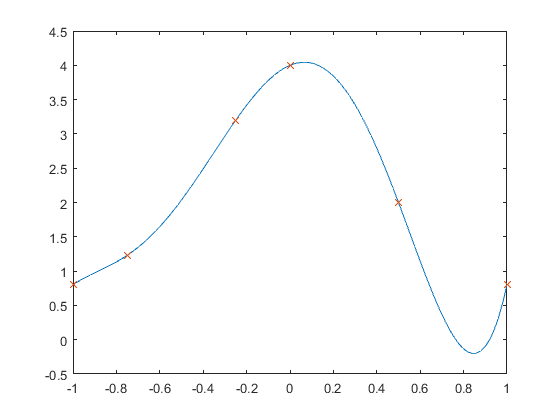
\includegraphics[width=0.7\textwidth]{figures/question1}
\end{center}

\section{}
\begin{center}
  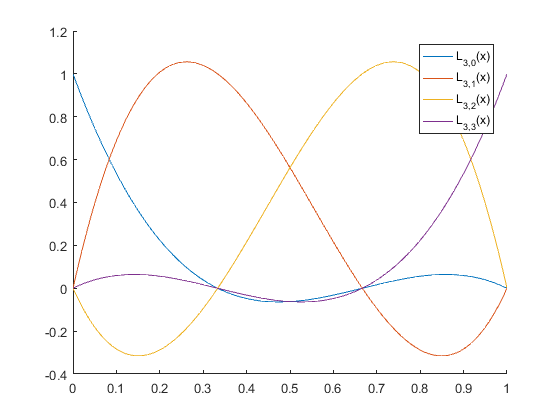
\includegraphics[width=0.7\textwidth]{figures/question2}
\end{center}

\section{}
\subsection*{a.}
\begin{center}
  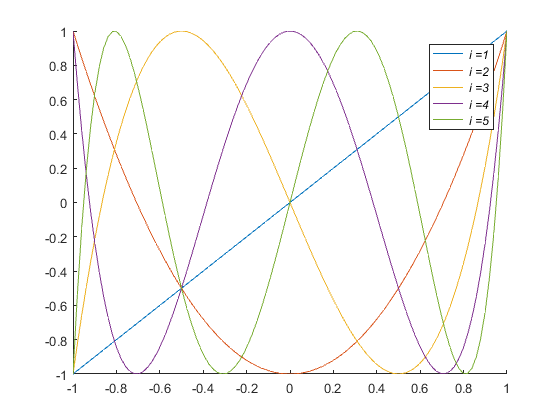
\includegraphics[width=0.7
    \textwidth]{figures/question3}
\end{center}
\subsection*{b.}
Show that \(T_n(x)=cos(n\cdot acos(x))\) is a polynomial of degree
\(n\).
\begin{enumerate}
\item First, we let \(\theta=acos(x)\), and consequently
  \(x=cos(\theta)\), and \(T_n(x)=cos(n\theta)\).
  \item Recall the identity
    \(cos\left((n+1)\theta\right)=2cos(\theta)cos(n\theta)-cos\left((n-1)\theta\right)\)
\item Using the previous identity, and plugging in \(x=cos(\theta)\)
  and \(T_n(x)=cos(n\theta)\) we get
  \(T_{n+1}=2xT_n -T_{n-1}\)
\end{enumerate}
Since \(T_0=1\), it follows by induction that the nth degree Chebyshev
polynomial has degree n.
\subsection*{c.}
Recall the trigonometric identity
\(cos\left((2k+1)\frac{\pi}{2}\right)=0\). Then to find the roots of
the Chebyshev polynomial we solve
\[cos\left(n\cdot acos(x)\right)=0\]
We use the identity to find
\[n\cdot acos(x) = (2k+1)\cdot\frac{\pi}{2}\]
then solve for x to find
\[\left\{\xi_i\right\}_{1\leq i\leq n}=cos\left(\frac{(2k+1)\pi}{2n}\right),\quad k=1,\dots,n\]


\pagebreak
\section{}
\subsection*{a.}
\begin{center}
  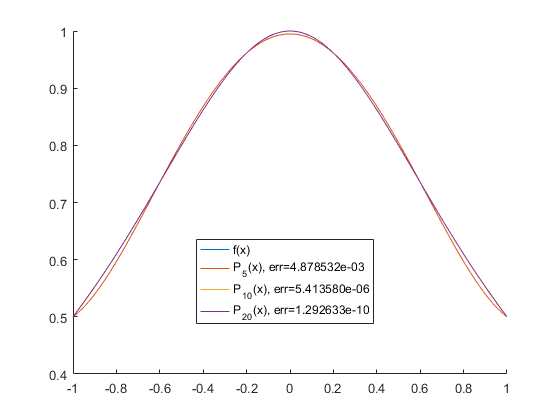
\includegraphics[width=0.8\linewidth]{figures/question4-1}
\end{center}
\begin{center}
  \begin{figure}[h!]
    \minipage{0.5\textwidth}
    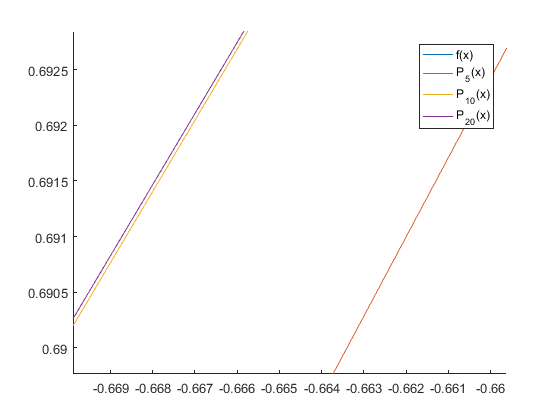
\includegraphics[width=\linewidth]{figures/question4-2}
    \endminipage\hfill
    \minipage{0.5\textwidth}
    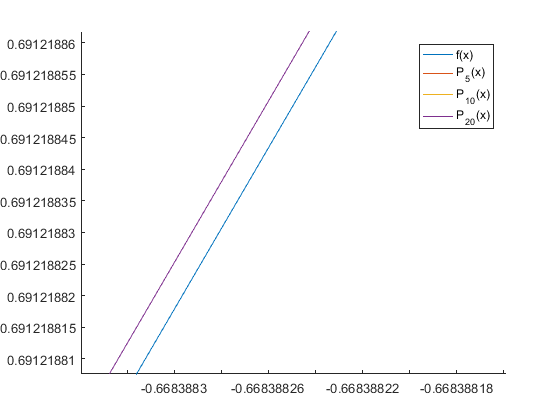
\includegraphics[width=\linewidth]{figures/question4-3}
    \endminipage
  \end{figure}
\end{center}
Considered on the scale from -1 to 1, even the 5th order polynomial is
a fairly good approximation. As you add more points it gets even
better, and the 20th order polynomial is nearly indistinguishable.\\
The error on the main plot is the sum of squared differences.
\subsection*{b.}
\begin{center}
    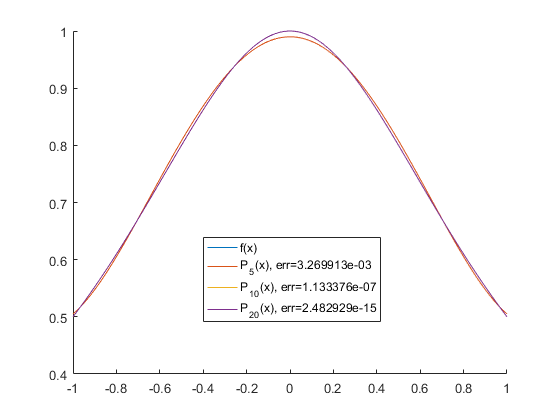
\includegraphics[width=0.7\linewidth]{figures/question4b.png}
\end{center}
As we can see, the interpolation using the Chebyshev nodes is more accurate. 
The error on the plot is the sum of squared differences, and it is less than
the plot in 4a.

\section{}
When given pairwise-distinct points \(\{x_0,x_1,\dots,x_n\}\), the
Newton interpolation of a function is
\[f(t) \approx f[x_0] + f[x_0,x_1](x-x_0) + \dots\]
Also, we know that evaluating the interpolation at any one of the
nodes gives us the correct answer. The error of the interpolation is
zero at each of the nodes.\\
We are given an interpolating polynomial \(P_n(t)\) plus the next
Newton interpolation term
\(f[x_0,x_1,\dots,x_n,t](t-x_0)\dots(t-x_n)\). This new function that
is the sum of the two is just another, better interpolation of
\(f(x)\), and since \(t\) is one of the nodes, we know that this
function will have zero error at \(t\). Thus
\[f(t)=P_n(t)+f[x_0,x_1,\dots,x_n,t](t-x_0)(t-x_1)\dots(t-x_n)\]


\end{document}
